% This report template is adapted from the ICLR 2026 LaTeX template.

\documentclass{article} % For LaTeX2e
\usepackage{report,times}

% Optional math commands from https://github.com/goodfeli/dlbook_notation.
\input{math_commands.tex}
\usepackage{graphicx}
\usepackage{subcaption}
\usepackage{hyperref}
\usepackage{url}
\usepackage{listings}

% this is adapted from from the source code of the ScholarCopilot paper published on arxiv.
\lstset{
    basicstyle=\ttfamily\small,      % 设定基础字体和字号
    columns=fullflexible,            % 更美观的宽度控制
    frame=single,                    % 单一边框
    breaklines=true,                 % 自动换行
    breakatwhitespace=true,          % 优先在空白处换行
    keepspaces=true,                 % 保留空格
    showspaces=false,                % 不显示空格标记
    showstringspaces=false,          % 字符串空格不显示特殊标记
    showtabs=false,                  % 不显示tab标记
    tabsize=4,                       % tab宽度
    rulecolor=\color{gray!50},       % 边框颜色
    backgroundcolor=\color{gray!5},  % 浅色背景
    language=[LaTeX]TeX,
    literate={\ \ }{{\ }}1,           % 改善空格显示
    numbers=none
}

\newcommand{\refsec}[1]{Sec. \ref{#1}}
\newcommand{\reffig}[1]{\figurename{ \ref{#1}}}
\newcommand{\refeq}[1]{Eq. \ref{#1}}
\newcommand{\refalg}[1]{Algo. \ref{#1}}
\newcommand{\reftab}[1]{Table \ref{#1}}
\newcommand{\reflst}[1]{Listing \ref{#1}}

\definecolor{commentgreen}{rgb}{0.5,0.5,0}
\definecolor{tablegray}{rgb}{0.95,0.95,0.95}
\newcommand{\note}[1]{\textcolor{commentgreen}{// #1}\\}% colored c-style comment
\newcommand{\mathnote}[1]{\textcolor{commentgreen}{\text{// #1}}}% for math env
\newcommand{\D}{\text{d}}% leibniz notation d for derivatives/integrals
\newcommand{\lp}[1]{\left({#1}\right)}% large parentheses, e.g. for vectors or fractions
\newcommand{\lpvar}[1]{\left\{{#1}\right\}}% large {} parentheses, e.g. for sets
\newcommand{\mono}[1]{\texttt{#1}}% monospace text

% TODO: Replace with your project title.
\title{Single View to Stereo Image Synthesis}

% TODO: Replace with your team members' names.
\author{
Niklas Munkes$^1$, Team Member2$^2$ \\
$^1$Media Informatics, $^2$Medieninformatik \\
\texttt{\{niklas.munkes, member2\}@student.uni-tuebingen.de}
}

\newcommand{\fix}{\marginpar{FIX}}
\newcommand{\new}{\marginpar{NEW}}
\begin{document}

\maketitle

\begin{figure}[htpb]
\centering
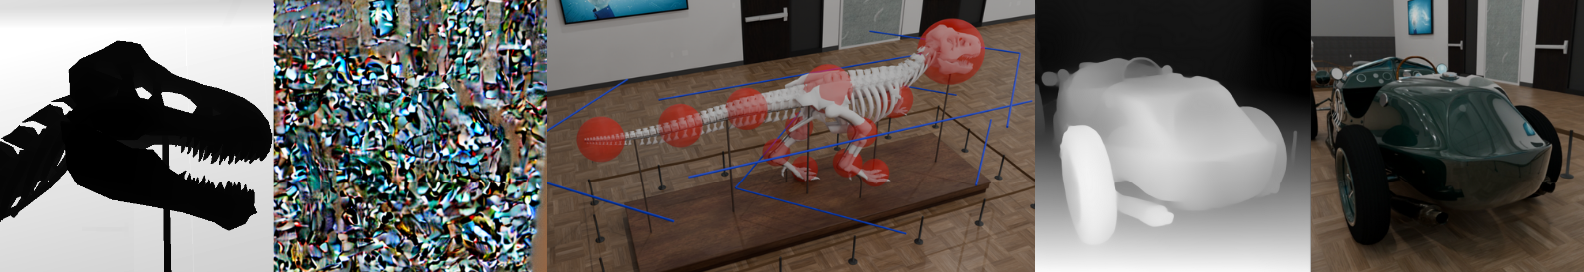
\includegraphics[clip,width=\textwidth]{figures/presentation_teaser.png}
% 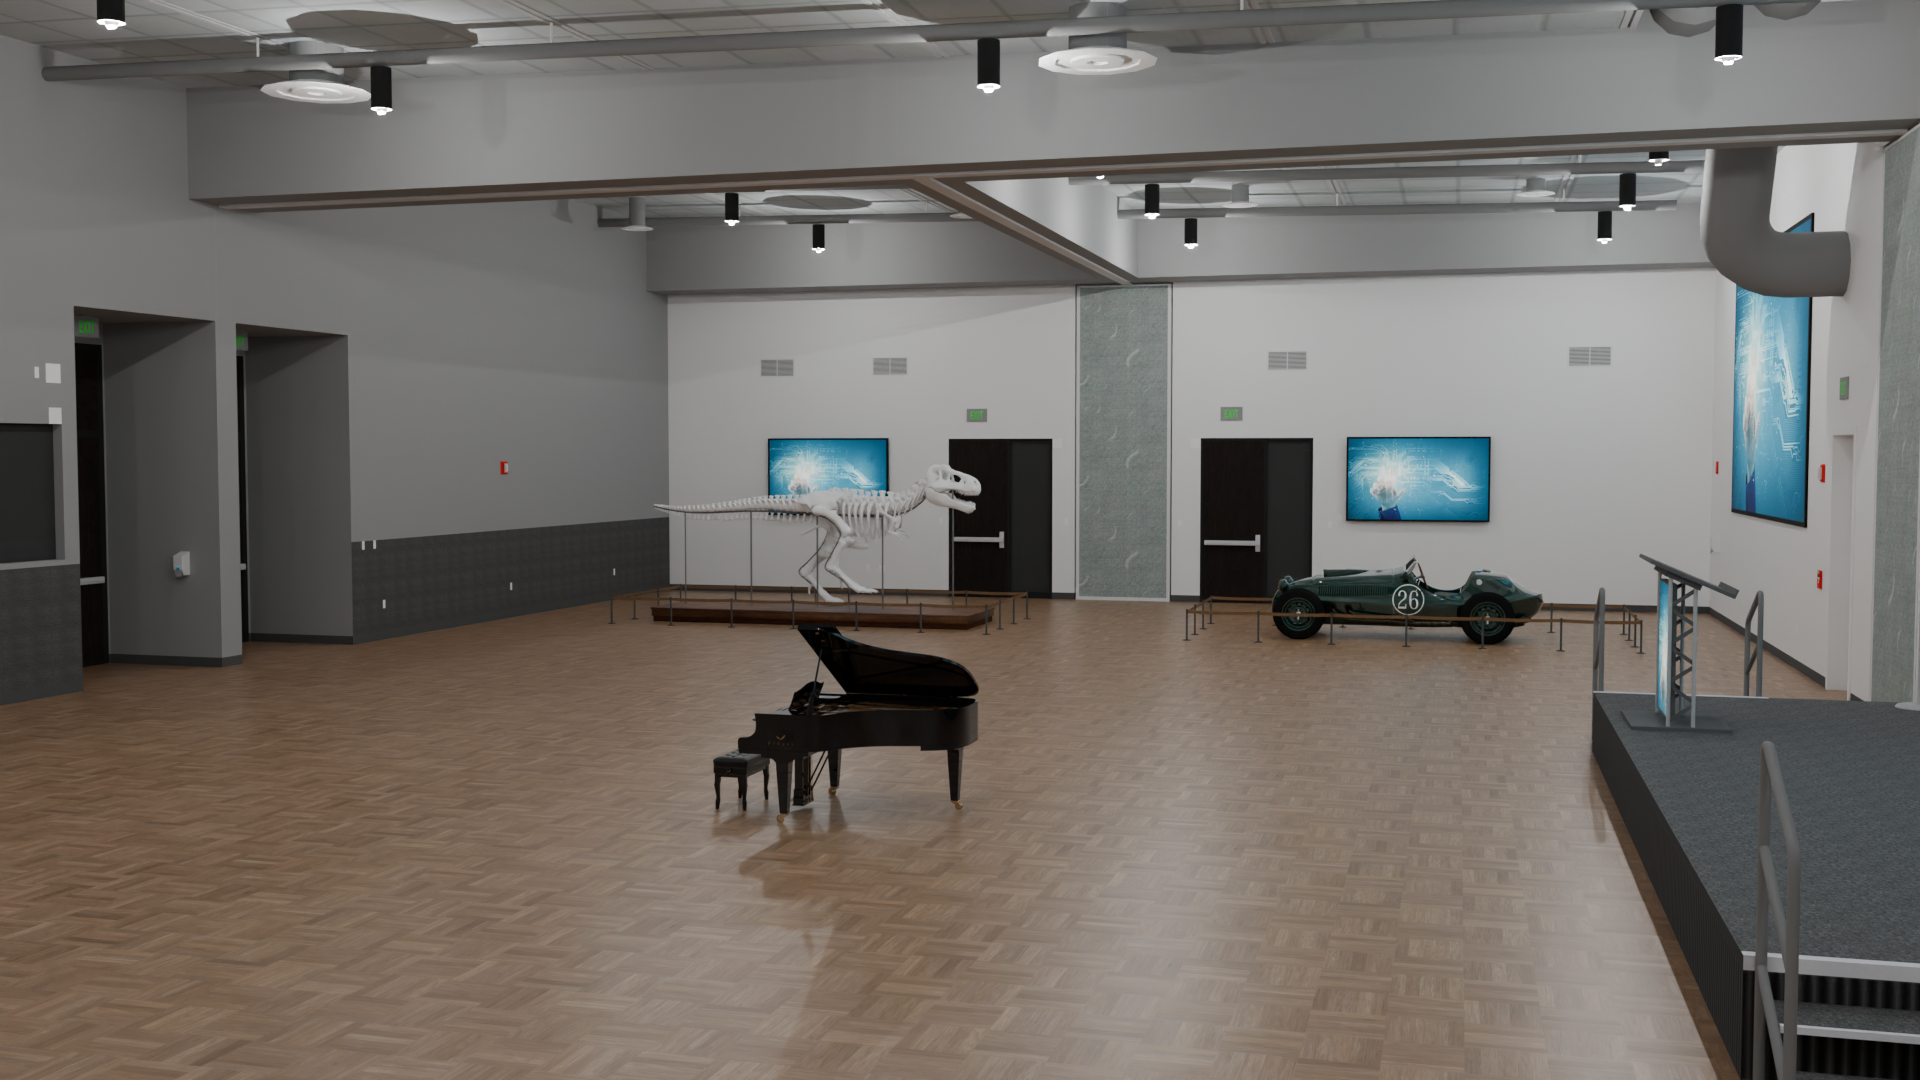
\includegraphics[trim=0 180 0 130,clip,width=\textwidth]{figures/preview_image_02.png}
% 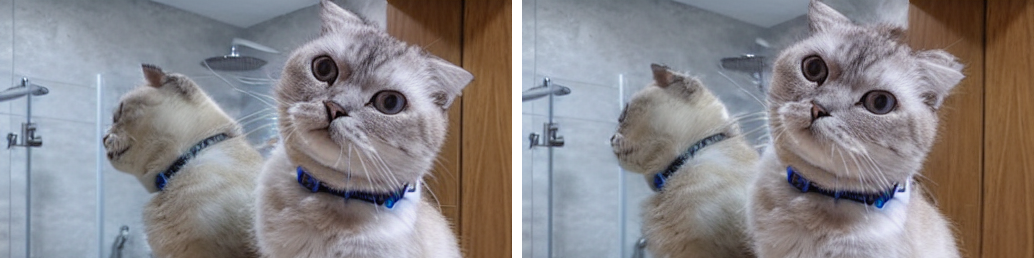
\includegraphics[clip,width=\textwidth]{figures/cats_halfheight.png}
% \caption{\textbf{Teaser.} TODO: Replace this placeholder with a teaser figure that summarizes your main result.}
\label{fig:teaser}
\end{figure}

\begin{abstract}
TODO

% The abstract paragraph should be indented 1/2~inch (3~picas) on both left and
% right-hand margins. Use 10~point type, with a vertical spacing of 11~points.
% The word \textsc{Abstract} must be centered, in small caps, and in point size 12. Two
% line spaces precede the abstract. The abstract must be limited to one
% paragraph.
\end{abstract}

\section{Methods}\label{methods}
% intro stereodiffusion
% TODO

In this work we investigate what impact different alterations of the StereoDiffusion \cite{Wang-2024-stereodiffusion} architecture have on its ability to generate stereo image pairs. Specifically, we propose and evaluate the following modifications to StereoDiffusion: (1) a method for ... (\refsec{depth-to-disparity})

\subsection{Disparity Computation}\label{depth-to-disparity}
TODO

\subsection{Cross-Attention}\label{cross-attn}
TODO

\subsection{Null-text Inversion}\label{null-text-inv}
TODO

\subsection{Ground-truth SPSMD}\label{gt-alignment}
TODO

\subsection{Custom Disparity Prediction}\label{disp-training}
TODO


% https://ieeexplore.ieee.org/abstract/document/6248074 / aus anderer src => https://www.cs.toronto.edu/~urtasun/publications/geiger_et_al_cvpr12.pdf
% https://arxiv.org/abs/2504.16930
% https://arxiv.org/abs/2403.04965
% https://arxiv.org/abs/1512.02134 not used

\section{Dataset}
For the evaluation process or training, a dataset is required. A dataset contains a pair of stereo images and a ground-truth depth / disparity map. There are mainly two options for creating such a dataset, either in the real-world with stereo image sensors or computer-generated synthetic data.

Therefore, there are two essential ways to create such a dataset: either in the real-world using stereo image sensors, or using computer-generated synthetic data.

\subsection{Real-World approach}
Creating a real-world dataset requires substantial resources and time. Stereo sensors are required and must be calibrated. The environment needs to be carefully selected, especially with regard to lighting. Motion in the scenes is also a significant challenge. Since the KITTI dataset was captured from a vehicle, 3D sensing accuracy was therefore particularly important \cite{6248074}.

\subsection{Synthetic approach}
Creating a dataset in a synthetic environment offers the greatest possibility. This can save considerable time and resources, especially when specialized scenes are required. Furthermore, because the dataset is generated in a synthetic environment, the depth / disparity map can provide more accurate ground-truth, since the computation is not based on approximated values.

\subsection{Our Solution}
We decided to create our own computer-generated synthetic dataset for several reasons. First if we use an existing dataset, we have no control over the scene composition. If it's a real-world based dataset, it may not contain depth / disparity map or only an approximate one. It is also unclear whether the dataset has already been used in an existing training process. If so the evaluation could be biased.

Creating our own synthetic dataset could also provide greater possibilities for camera setups, if required in later training or evaluation. This would be much more difficult to achieve with a real-world camera setup.

As a render engine we used Blender. We set up a custom scene and a stereo rendering system. \\
In our initial approach, we generated the scene in a random, simple procedurally way figure \ref{fig:procedural_approach}. The limitations of this initial approach were the low complexity of the given primitives and the scene overall. Also the level of complexity within the distance / background was too low \cite{yan2026makesgoodsynthetictraining}. To address these issues in consideration with our very limited resources and time, the new scene, shown in figure \ref{fig:improved_approach}, consists of some specially selected objects with different surface characteristics. These objects were specifically positioned in the scene and in combination with the background, they provide different levels of surface characteristics on different distances.

\subsubsection{Generation}
Our stereo rendering system consists of three stages. The first stage is the camera initialization. To get the capability to render a large number of images, we created a procedural stereo camera system, shown in Figure \ref{fig:camera_initialization}. This system consists of two tasks. \\
\\
In the first task, we define multiple POIs for each Object of interest. These points of interest are used to orient the cameras towards the nearest POI. Second, we create camera paths around each object of interest. Cameras are later automatically placed along these paths by a script. The script then distributes a specified number of cameras evenly along the paths. \\
\\
The second stage is the stereo image rendering and the associated depth map generating within in Blender. This is done using another script that iterates over the pre-initialized cameras. For each camera, the script creates a temporary stereo camera configuration with randomly parameters within predefined bounds. Based on this configuration the stereo image pairs are rendered. In this process, the baseline and focal length are randomized. In addition, the depth map is generated for the left image (EXR format). \\
The lighting, objects and materials remain static throughout the entire creation process and are therefore not automatically randomized. \\
\\
The third stage consists of disparity map generation, which is a separate process outside of Blender. Therefore, a separate script is used to generate the corresponding disparity map (EXR format) for each sample. \\
\\
The following formula was used for this \cite{Wang-2024-stereodiffusion}: \\
$D(x,y)=\frac{fB}{Z(x,y)}$
\\
\\
Our dataset consists of four main objects. For each of these main objects, 1000 samples were generated. Each sample consists of a pair of stereo images with a resolution of 512$\times$512 pixels, along with the corresponding disparity map, depth map, and metadata. Due to the large amount of data, we decided to use JPG compression.

\subsubsection{Example}
Figure \ref{fig:dino_example} shows a sample of our dataset. \\
The stereo configuration parameters are as follows: \\
Baseline: 0.1 m \\
Focal Length: 38.4 mm \\

\begin{figure}[htpb]
    \centering
    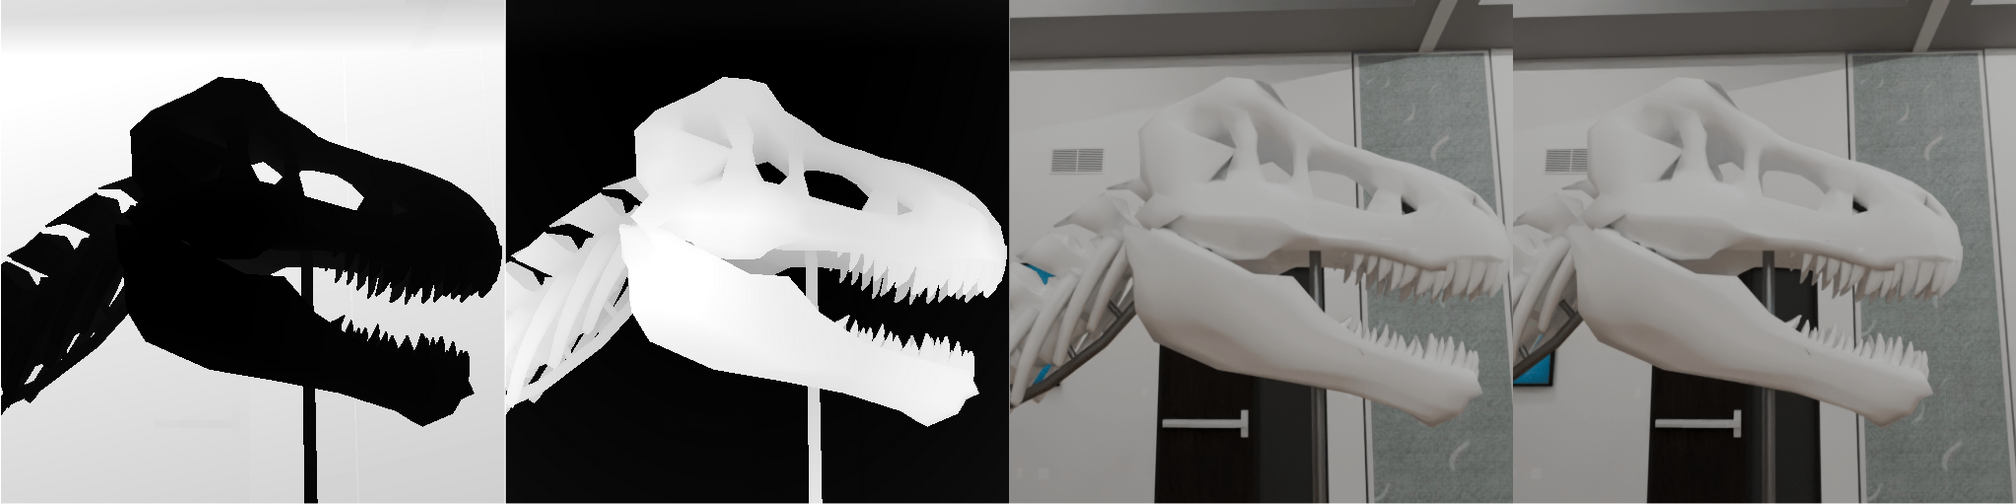
\includegraphics[width=1.0\linewidth]{figures/dino_example.png}
    \caption{Example sample - depth map, disparity map, left image, right image}
    \label{fig:dino_example}
\end{figure}

% left/right?
\section{Experiments}\label{experiments}
TODO

\label{fig:quality-right-mean} % bitte der betreffenden figure hinzufügen!
\label{fig:left-vs-right-ssim} % bitte der betreffenden figure hinzufügen!

% \section{General Instructions}

% The final report should present your project findings in the style of a scientific paper. We strongly encourage a rigorous, scientific writing style. Reports that are well-structured, clearly written, and objectively argued will be evaluated more favorably.

% \subsection{Expectations}

% Please keep the following expectations in mind while writing:
% \begin{itemize}
%   \item \textbf{Clear problem statement and contribution:} Clearly state the task, assumptions, and the main contributions of your project.
%   \item \textbf{Related work and references:} Use proper citations throughout. References are crucial to demonstrate awareness of the field and to position your method relative to prior work.
%   \item \textbf{Detailed method:} Describe your method in sufficient detail so that a reader can clearly understand how you solve the problem.
%   \item \textbf{Evaluation tasks:} Design evaluation tasks that meaningfully test your solution. If applicable, motivate why these tasks reflect the problem you aim to solve.
%   \item \textbf{Baselines / comparisons:} Where possible, compare against an existing method, a reasonable baseline, or an ablation/alternative variant of your approach. Explain what you learn from these comparisons.
%   \item \textbf{Quantitative + qualitative evidence:} In addition to qualitative examples, include at least one quantitative metric aligned with your problem formulation (e.g., accuracy, user-study scores, or other task-specific measures) and report it consistently.
%   \item \textbf{Results and interpretation:} Present results clearly in tables and figures, and interpret them. Discuss strengths, limitations, and failure cases.
%   \item \textbf{Novel findings:} Highlight any novel insights, unexpected observations, or lessons learned during the project.
% \end{itemize}

% \subsection{Length}
% The report length does not necessarily correlate with its quality. \textbf{5--8 pages (excluding references)} should be sufficient to present your work.

% \subsection{Style}
% Authors must use the provided \LaTeX{} style files available on the course page on \textbf{ILIAS}. Do not change any formatting parameters in the style files. In particular, do not modify the text area (i.e., the width or height of the page layout), and do not change font sizes (except possibly in the \textsc{References} section; see below). Please ensure that pages are numbered. For guidance on citations, figures, and tables, please refer to \sectionautorefname~\ref{sec_others}. For mathematical notation and equation writing, please refer to \sectionautorefname~\ref{sec_notation}.

% \subsection{Visualization}
% Visualizations are strongly encouraged, including:
% \begin{itemize}
%     \item A \textbf{teaser figure} that summarizes your main result (key selling point).
%     \item A \textbf{pipeline/overview figure} that illustrates your method.
%     \item \textbf{Qualitative result figures} that showcase typical outcomes as well as failure cases (if applicable).
% \end{itemize}

% \section{Author Contributions}
% This section is mandatory. Please clearly describe the contribution of each team member (e.g., conceptualization, implementation, experiments, analysis, writing). You may choose to complete this section at the end of the report.

% \section{Citations, figures, tables, references}
% \label{sec_others}

% \subsection{Citations within the text}

% Citations within the text should be based on the \texttt{natbib} package
% and include the authors' last names and year (with the ``et~al.'' construct
% for more than two authors). When the authors or the publication are
% included in the sentence, the citation should not be in parenthesis using \verb|\citet{}| (as
% in ``See \citet{Hinton06} for more information.''). Otherwise, the citation
% should be in parenthesis using \verb|\citep{}| (as in ``Deep learning shows promise to make progress
% towards AI~\citep{Bengio+chapter2007}.'').

% The corresponding references are to be listed in alphabetical order of
% authors, in the \textsc{References} section. As to the format of the
% references themselves, any style is acceptable as long as it is used
% consistently.

% \subsection{Footnotes}

% Indicate footnotes with a number\footnote{Sample of the first footnote} in the
% text. Place the footnotes at the bottom of the page on which they appear.
% Precede the footnote with a horizontal rule of 2~inches
% (12~picas).\footnote{Sample of the second footnote}

% \subsection{Figures}

% All artwork must be neat, clean, and legible. Lines should be dark
% enough for purposes of reproduction; art work should not be
% hand-drawn. The figure number and caption always appear after the
% figure. Place one line space before the figure caption, and one line
% space after the figure. The figure caption is lower case (except for
% first word and proper nouns); figures are numbered consecutively.

% Make sure the figure caption does not get separated from the figure.
% Leave sufficient space to avoid splitting the figure and figure caption.

% You may use color figures.
% However, it is best for the
% figure captions and the paper body to make sense if the paper is printed
% either in black/white or in color.
% \begin{figure}[h]
% \begin{center}
% %\framebox[4.0in]{$\;$}
% \fbox{\rule[-.5cm]{0cm}{4cm} \rule[-.5cm]{4cm}{0cm}}
% \end{center}
% \caption{Sample figure caption.}
% \end{figure}

% \subsection{Tables}

% All tables must be centered, neat, clean and legible. Do not use hand-drawn
% tables. The table number and title always appear before the table. See
% \tableautorefname~\ref{sample-table}.

% Place one line space before the table title, one line space after the table
% title, and one line space after the table. The table title must be lower case
% (except for first word and proper nouns); tables are numbered consecutively.

% \begin{table}[t]
% \caption{Sample table title}
% \label{sample-table}
% \begin{center}
% \begin{tabular}{ll}
% \multicolumn{1}{c}{\bf PART}  &\multicolumn{1}{c}{\bf DESCRIPTION}
% \\ \hline \\
% Dendrite         &Input terminal \\
% Axon             &Output terminal \\
% Soma             &Cell body (contains cell nucleus) \\
% \end{tabular}
% \end{center}
% \end{table}

% \section{Default Notation}
% \label{sec_notation}
% In an attempt to encourage standardized notation, we have included the
% notation file from the textbook, \textit{Deep Learning}
% \cite{goodfellow2016deep} available at
% \url{https://github.com/goodfeli/dlbook_notation/}.  Use of this style
% is not required and can be disabled by commenting out
% \texttt{math\_commands.tex}.


% \centerline{\bf Numbers and Arrays}
% \bgroup
% \def\arraystretch{1.5}
% \begin{tabular}{p{1in}p{3.25in}}
% $\displaystyle a$ & A scalar (integer or real)\\
% $\displaystyle \va$ & A vector\\
% $\displaystyle \mA$ & A matrix\\
% $\displaystyle \tA$ & A tensor\\
% $\displaystyle \mI_n$ & Identity matrix with $n$ rows and $n$ columns\\
% $\displaystyle \mI$ & Identity matrix with dimensionality implied by context\\
% $\displaystyle \ve^{(i)}$ & Standard basis vector $[0,\dots,0,1,0,\dots,0]$ with a 1 at position $i$\\
% $\displaystyle \text{diag}(\va)$ & A square, diagonal matrix with diagonal entries given by $\va$\\
% $\displaystyle \ra$ & A scalar random variable\\
% $\displaystyle \rva$ & A vector-valued random variable\\
% $\displaystyle \rmA$ & A matrix-valued random variable\\
% \end{tabular}
% \egroup
% \vspace{0.25cm}

% \centerline{\bf Sets and Graphs}
% \bgroup
% \def\arraystretch{1.5}

% \begin{tabular}{p{1.25in}p{3.25in}}
% $\displaystyle \sA$ & A set\\
% $\displaystyle \R$ & The set of real numbers \\
% $\displaystyle \{0, 1\}$ & The set containing 0 and 1 \\
% $\displaystyle \{0, 1, \dots, n \}$ & The set of all integers between $0$ and $n$\\
% $\displaystyle [a, b]$ & The real interval including $a$ and $b$\\
% $\displaystyle (a, b]$ & The real interval excluding $a$ but including $b$\\
% $\displaystyle \sA \backslash \sB$ & Set subtraction, i.e., the set containing the elements of $\sA$ that are not in $\sB$\\
% $\displaystyle \gG$ & A graph\\
% $\displaystyle \parents_\gG(\ervx_i)$ & The parents of $\ervx_i$ in $\gG$
% \end{tabular}
% \vspace{0.25cm}


% \centerline{\bf Indexing}
% \bgroup
% \def\arraystretch{1.5}

% \begin{tabular}{p{1.25in}p{3.25in}}
% $\displaystyle \eva_i$ & Element $i$ of vector $\va$, with indexing starting at 1 \\
% $\displaystyle \eva_{-i}$ & All elements of vector $\va$ except for element $i$ \\
% $\displaystyle \emA_{i,j}$ & Element $i, j$ of matrix $\mA$ \\
% $\displaystyle \mA_{i, :}$ & Row $i$ of matrix $\mA$ \\
% $\displaystyle \mA_{:, i}$ & Column $i$ of matrix $\mA$ \\
% $\displaystyle \etA_{i, j, k}$ & Element $(i, j, k)$ of a 3-D tensor $\tA$\\
% $\displaystyle \tA_{:, :, i}$ & 2-D slice of a 3-D tensor\\
% $\displaystyle \erva_i$ & Element $i$ of the random vector $\rva$ \\
% \end{tabular}
% \egroup
% \vspace{0.25cm}


% \centerline{\bf Calculus}
% \bgroup
% \def\arraystretch{1.5}
% \begin{tabular}{p{1.25in}p{3.25in}}
% % NOTE: the [2ex] on the next line adds extra height to that row of the table.
% % Without that command, the fraction on the first line is too tall and collides
% % with the fraction on the second line.
% $\displaystyle\frac{d y} {d x}$ & Derivative of $y$ with respect to $x$\\ [2ex]
% $\displaystyle \frac{\partial y} {\partial x} $ & Partial derivative of $y$ with respect to $x$ \\
% $\displaystyle \nabla_\vx y $ & Gradient of $y$ with respect to $\vx$ \\
% $\displaystyle \nabla_\mX y $ & Matrix derivatives of $y$ with respect to $\mX$ \\
% $\displaystyle \nabla_\tX y $ & Tensor containing derivatives of $y$ with respect to $\tX$ \\
% $\displaystyle \frac{\partial f}{\partial \vx} $ & Jacobian matrix $\mJ \in \R^{m\times n}$ of $f: \R^n \rightarrow \R^m$\\
% $\displaystyle \nabla_\vx^2 f(\vx)\text{ or }\mH( f)(\vx)$ & The Hessian matrix of $f$ at input point $\vx$\\
% $\displaystyle \int f(\vx) d\vx $ & Definite integral over the entire domain of $\vx$ \\
% $\displaystyle \int_\sS f(\vx) d\vx$ & Definite integral with respect to $\vx$ over the set $\sS$ \\
% \end{tabular}
% \egroup
% \vspace{0.25cm}

% \centerline{\bf Probability and Information Theory}
% \bgroup
% \def\arraystretch{1.5}
% \begin{tabular}{p{1.25in}p{3.25in}}
% $\displaystyle P(\ra)$ & A probability distribution over a discrete variable\\
% $\displaystyle p(\ra)$ & A probability distribution over a continuous variable, or over
% a variable whose type has not been specified\\
% $\displaystyle \ra \sim P$ & Random variable $\ra$ has distribution $P$\\% so thing on left of \sim should always be a random variable, with name beginning with \r
% $\displaystyle  \E_{\rx\sim P} [ f(x) ]\text{ or } \E f(x)$ & Expectation of $f(x)$ with respect to $P(\rx)$ \\
% $\displaystyle \Var(f(x)) $ &  Variance of $f(x)$ under $P(\rx)$ \\
% $\displaystyle \Cov(f(x),g(x)) $ & Covariance of $f(x)$ and $g(x)$ under $P(\rx)$\\
% $\displaystyle H(\rx) $ & Shannon entropy of the random variable $\rx$\\
% $\displaystyle \KL ( P \Vert Q ) $ & Kullback-Leibler divergence of P and Q \\
% $\displaystyle \mathcal{N} ( \vx ; \vmu , \mSigma)$ & Gaussian distribution %
% over $\vx$ with mean $\vmu$ and covariance $\mSigma$ \\
% \end{tabular}
% \egroup
% \vspace{0.25cm}

% \centerline{\bf Functions}
% \bgroup
% \def\arraystretch{1.5}
% \begin{tabular}{p{1.25in}p{3.25in}}
% $\displaystyle f: \sA \rightarrow \sB$ & The function $f$ with domain $\sA$ and range $\sB$\\
% $\displaystyle f \circ g $ & Composition of the functions $f$ and $g$ \\
%   $\displaystyle f(\vx ; \vtheta) $ & A function of $\vx$ parametrized by $\vtheta$.
%   (Sometimes we write $f(\vx)$ and omit the argument $\vtheta$ to lighten notation) \\
% $\displaystyle \log x$ & Natural logarithm of $x$ \\
% $\displaystyle \sigma(x)$ & Logistic sigmoid, $\displaystyle \frac{1} {1 + \exp(-x)}$ \\
% $\displaystyle \zeta(x)$ & Softplus, $\log(1 + \exp(x))$ \\
% $\displaystyle || \vx ||_p $ & $\normlp$ norm of $\vx$ \\
% $\displaystyle || \vx || $ & $\normltwo$ norm of $\vx$ \\
% $\displaystyle x^+$ & Positive part of $x$, i.e., $\max(0,x)$\\
% $\displaystyle \1_\mathrm{condition}$ & is 1 if the condition is true, 0 otherwise\\
% \end{tabular}
% \egroup
% \vspace{0.25cm}

% \section{Preparing for submission}

% The deadline for submitting the final report is \textbf{23:59 (CET), 31 March 2026}. Please submit a \textbf{PDF} version via \textbf{ILIAS}.

\newpage
\bibliography{report}
\bibliographystyle{report}
\input{sections/credits.tex}

\newpage
\appendix
\section{Supplementary Material}\label{appendix}
% if anyone has additional things to show (e.g. evaluation that got cut (eval6), our old geometric shapes dataset, etc.), put that stuff here.

% eval6 (training)
\subsection{Trained Disparity Estimation Model}\label{trained-disparity}
TODO (maybe)

% focal length/baseline distance via prompt+qwen

% \subsection{Example: Different Interpretation of Shifted Content}\label{reinterpreted-shifted}
% TODO % gt left, gt right, gen right
% \begin{figure}[htb]
%     \centering
%     \begin{subfigure}[b]{0.32\linewidth}
%     \includegraphics[width=\linewidth]{../../latex_template/ex06/images/06-2_midirect-ref.png}
%     \caption{reference}
%     \end{subfigure}
%     \begin{subfigure}[b]{0.32\linewidth}
%     \includegraphics[width=\linewidth]{../../nori/scenes/ex06/veach_mi/veach_mi-midirect-uniform.png}
%     \caption{result (with uniform heuristic)}
%     \end{subfigure}
%     \begin{subfigure}[b]{0.32\linewidth}
%     \includegraphics[width=\linewidth]{../../latex_template/ex06/images/06-2_midirect-uniform-diff.png}
%     \caption{difference}
%     \end{subfigure}
%     \caption*{Comparison for \ref{6.2} a)}
% \end{figure}

\end{document}
